 O dispositivo experimental usado para produzir eletricidade, a partir de uma reação espontânea, é designado por célula galvânica ou célula voltaica, em homenagem aos cientistas italianos Luigi Galvani e Alessandro Volta, que construíram os primeiros protótipos do dispositivo. O potencial da célula para a célula voltaica esquematizada abaixo é de 0,109 V, sob condições padrão, 1 mol$\cdot$L$^{-1}$ de \chemfig{Ni^{2+}}(aq) e 1 mol$\cdot$L$^{-1}$ \chemfig{Pb^{2+}}(aq). Que alteração nesta célula poderia causar um aumento na diferença de potencial entre os eletrodos?

\begin{center}
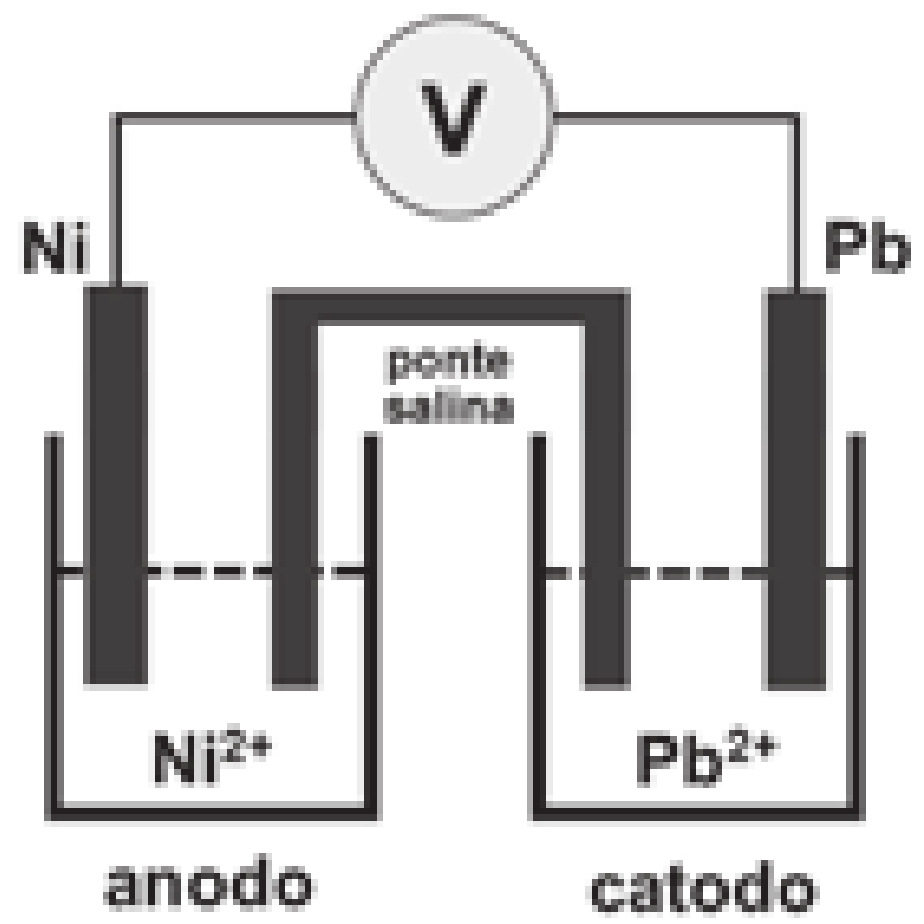
\includegraphics[width=0.25\textwidth]{figure.png}
\end{center}

\begin{enumerate}[label = (\alph*)]
	\item Adicionar mais solução de 1 mol$\cdot$L$^{-1}$ de \chemfig{Pb^{2+}} a essa semicélula.
	\item Usar um eletrodo de \chemfig{Ni} com maior massa. 
	\item Adicionar 50 mL de uma solução 1 mol$\cdot$L$^{-1}$ de \chemfig{NaCl} para precipitar \chemfig{PbCl}
	\item Diluir com \chemfig{H_2O} a solução de 1mol$\cdot$L$^{-1}$ de \chemfig{Ni_{2+}}
	\item Usar um elétrodo de \chemfig{Pb} com maior massa.
\end{enumerate}
